The derivation follows the infinitesimal-element analysis in the course notes~\cite[pp.~141--145]{Giurgiutiu2026Vibration}.

\textbf{1. Tension assumption.} The tension magnitude $T$ is constant along the string and does not change during small transverse vibration.

\textbf{2. Free-body diagram.} The tension vectors act tangentially and outward on the element. The net transverse force is
\[
\sum F_y=T\sin(\alpha+d\alpha)-T\sin\alpha.
\]
\begin{figure}[H]
\centering
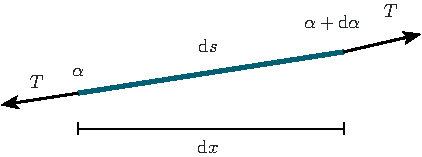
\includegraphics[width=0.62\linewidth]{figures/generated/solutions/A1-element.pdf}
\caption{Tension forces on an infinitesimal string element.}
\end{figure}

\textbf{3--5. Small-displacement approximation.} With $|u_x|\ll1$, $ds\simeq dx$, $\alpha\simeq u_x$, $\sin\alpha\simeq\alpha$, and $\sin(\alpha+d\alpha)\simeq\alpha+d\alpha$. Thus
\[
\sum F_y\simeq T\,d\alpha,\qquad d\alpha=\frac{\partial^2u}{\partial x^2}\,dx.
\]

\textbf{6--9. Newton's law and wave equation.} The element mass is $m\,dx$, where $m$ denotes mass per unit length. Dividing the force balance by $dx$ gives
\[
T u_{xx}=m u_{tt},\qquad c=\sqrt{\frac{T}{m}},\qquad \boxed{u_{tt}=c^2u_{xx}}.
\]

\textbf{10--14. Spatial differential equation.} Substituting $u=U(x)e^{-i\omega t}$ and cancelling the time factor gives
\[
U''+\frac{\omega^2}{c^2}U=0,\qquad
\gamma=\frac{\omega}{c},\qquad U''+\gamma^2 U=0.
\]
For $U=e^{sx}$, the characteristic equation is $s^2+\gamma^2=0$ and its roots are $s_1=i\gamma$ and $s_2=-i\gamma$.

\textbf{15--18. General solution.} The exponential and trigonometric spatial solutions are equivalent by Euler's formula,
\[
U=A_1e^{i\gamma x}+A_2e^{-i\gamma x}
 =C_1\sin(\gamma x)+C_2\cos(\gamma x).
\]
Restoring the prescribed harmonic factor gives
\[
\boxed{u(x,t)=[C_1\sin(\gamma x)+C_2\cos(\gamma x)]e^{-i\omega t}
=A_1e^{i(\gamma x-\omega t)}+A_2e^{-i(\gamma x+\omega t)}.}
\]
The first exponential travels in the positive $x$ direction and the second travels in the negative $x$ direction. The physical displacement is the real part.
